\documentclass{article}
\usepackage[utf8]{inputenc}
\usepackage{graphicx}
\graphicspath{ {images/} }

%----------------------------------------------------------------------------------------
%	TITLE PAGE
%----------------------------------------------------------------------------------------

\newcommand*{\titleGP}{\begingroup
\centering 
\vspace*{\baselineskip}

\rule{\textwidth}{1.6pt}\vspace*{-\baselineskip}\vspace*{2pt}
\rule{\textwidth}{0.4pt}\\[\baselineskip]

{\LARGE NavUP\\ [0.3\baselineskip] Architectural Requirements, Specifications and Design } \\ [0.2\baselineskip]
\rule{\textwidth}{0.4pt}\vspace*{-\baselineskip}\vspace{3.2pt}
\rule{\textwidth}{1.6pt}\\[\baselineskip] %

% \scshape %
% A concise specification on the functional requirements  \\
% and use cases of NavUP \\[\baselineskip]

% \vspace*{2\baselineskip}

Compiled By \\[\baselineskip]
{\Large Boikanyo Modiko - u15227678 \\
Linda Potgieter - u14070091 \\
Marthinus Richter - u15160671 \\
Nkosenhle Ncube - u13247914 \\ 
Quinton Swanepoel - u15245510 \\
Ruan Klinkert - u14022282\par} 

\vfill

{\scshape 201} \\[0.3\baselineskip]
{\large TEAM Tlc}\par

\endgroup}

\begin{document}


\titleGP

\newpage

\section{Introduction}

\subsection{Deliverable}
We are required to use the high level functional requirements of the NavUp system given in a separate document to identify the architectural design specifications that satisfy the identified functional requirements from our last assignment, focusing on the subsystems architectural designs.
\subsection{Scope}
The final objective is to create a NavUP mobile application as well as a web-based interface. The NavUP mobile app should be available on both android and ios platforms while the web-based interface will be used for administration and maintenance. The primary objective of NavUP is to allow students, visitors and staff to successfully navigate around campus in a efficient manner.

\subsection{Definitions, Acronyms and Abbreviations}

\begin{table}[ht!]
	
	\centering
	\begin{tabular}{|p{4cm}|p{7cm}|}
		\hline
		\textbf{Term} & \textbf{Definition} \\		
		\hline
        App & Mobile application \\
		\hline
		CRUD & Create, Read, Update and Delete \\
		\hline
		GPS & Global Positioning System \\
		\hline
		TUCBW & This Use Case Begins With \\
		\hline
		TUCEW & This Use Case Ends With \\
		\hline
		UP & University of Pretoria \\
		\hline
	\end{tabular}
\end{table}

\section{Overall Architectural Design}
\subsection{Overview}
\subsection{Deployment Diagram}

\pagebreak
\begin{figure}
\includegraphics[width=\textwidth]{deployment_diagram2}
\caption{Deployment diagram}
\end{figure}

\section{User Management Module}

\subsection{UML Class Diagram}
\includegraphics[width=\textwidth]{user_management_system_Class_diagram}


\subsection{Use Case Diagram}

\includegraphics[width=\textwidth]{user_management_system_Use_Case_diagram}

\subsection{Architectural Design of Module}
\paragraph{}The user management module will handle the login and registration of various users, namely Admin Users, Registered Users, and Guest Users. Guest users will still be able login into and make use of the NavUP system without registering but no data will saved on the system for them. The system stores all registered users' details including those from other modules.

\paragraph{}The user management system makes use of two major design patterns, Template and Memento. The inheritance between user and the types of users demonstrates the template design pattern. The registration class acts as the originator to create objects of type user in the system;the user acts as the memento storing a state object for each class; the user manager is the caretaker for the memento. This shows the how the memento pattern is implememtened.The UserState class is used to define the objects that will hold state data that is unique to each user, such as, steps taken, places visited, events attended and other attributes that will be brought foward by extra modules that are added to the system.

\paragraph{}This module connects to the notifications module, events modules and other add-on modules. Notifiactions are dependant on the user/s to which they are to be sent and hence there is a dependency present between these modules.The events module requires an admin user to instantiate and manage the event. One admin user may manage many events, but an event may only be managed by one admin user. 

\subsection{Technologies Used}
\paragraph{}A MySQL database will be used to manage basic user activities such as registration, authentication, and user privileges. The database will store information regarding all users and how each user should be able to interact with the system. This database should interlink with the ios, android, and web platforms.

\paragraph{}The admin user should be able to perform basic CRUD operations such as adding and removing users, creating events, and updating details regarding points of interest. 

\subsection{Non-Trivial Implementation Tasks}

%%%%%%%
%Ruan Klinkert - 14022282
%Points of Interest
\section{Points of Interest Module}

\subsection{UML Class Diagram}

\begin{figure}[!htb]
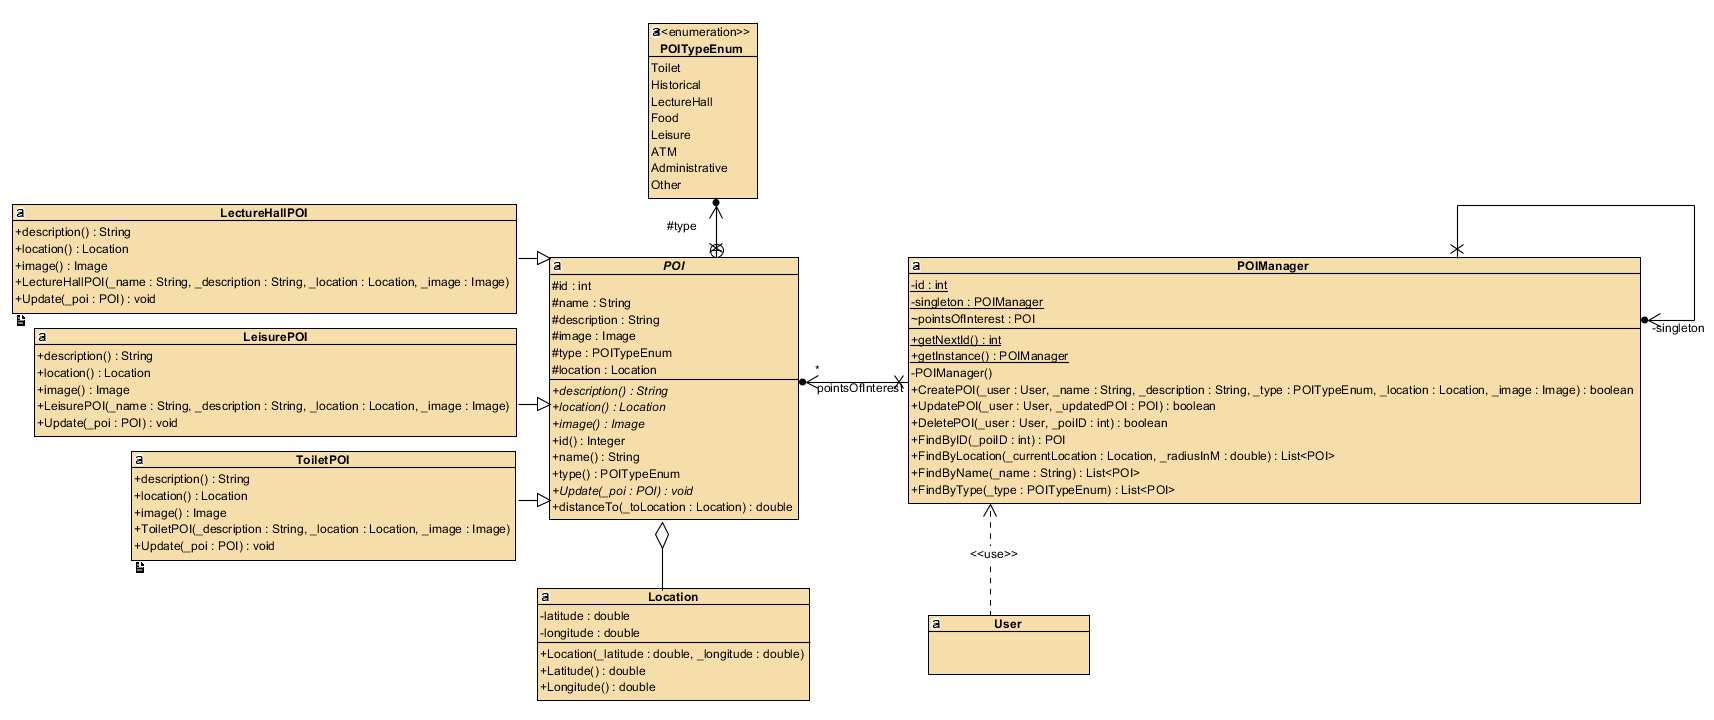
\includegraphics[width=\textwidth]{Images/ClassDiagram.png}
\caption{Class Diagram for the Points of interest module}
\end{figure}

\subsection{Use Case Diagram}

\begin{figure}[!htb]
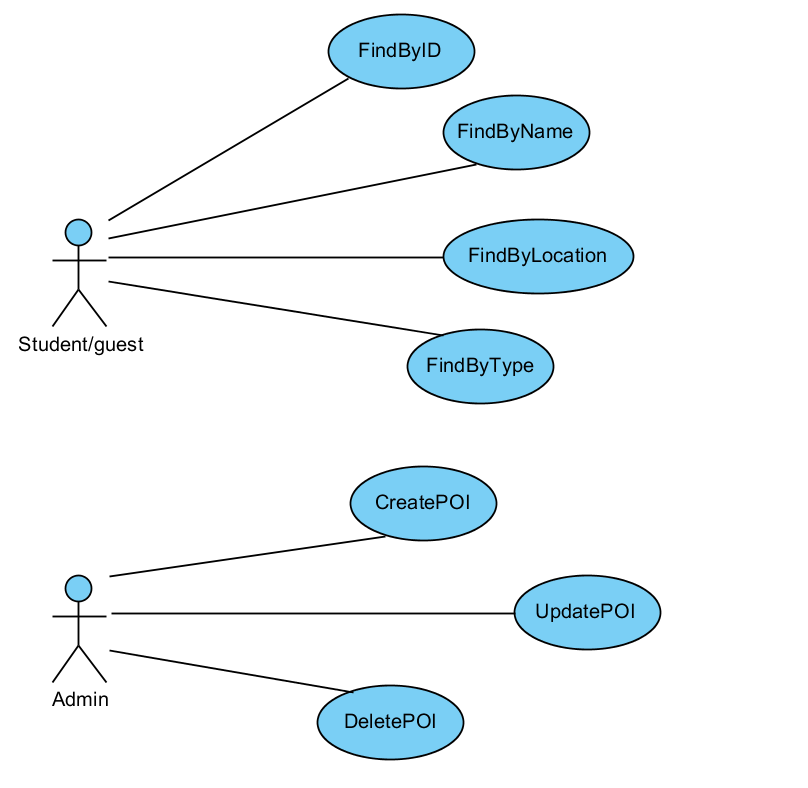
\includegraphics[width=\textwidth]{Images/UseCase.png}
\caption{Use Case Diagram for the Points of interest module}
\end{figure}

\subsection{Architectural Design of Module}

\paragraph{}The Points of Interest module will be used to persist and deliver data regarding locations that a user 
might find of interest. It will interact with the Events module, as well as the GIS module in order to retrieve and 
save it geographical location.

\paragraph{}One can assume that different types of Points of Interest(POI) will have different fields, constraints 
and requirements, therefore the POI module will make use of the factory design pattern, in order to create objects 
without exposing the creation logic to the client and allow us to refer to the newly created object using a common interface.

\paragraph{}The Points of Interest Manager class will make use of the Singleton design pattern to ensure that only one 
instance of the class exists, it will also act as the factory class to the points of interest class.

\paragraph{}At the core a Point of Interest object will have a location, description, unique id, type, name and image. 
The concrete object will then be able to impose additional attributes and constraints, such as Gender for bathrooms for 
example.

\paragraph{}Finally, the abstract point of interest class will be equipped with a stringify function to get a JSON 
representation of the object. 

\subsection{Technologies Used}

\paragraph{}It can be assumed that different types of Points of Interest will have different fields, constraints and 
requirements, therefore a traditional relational database will not be suitable for this type of data. Hence we will 
rather go for a document-oriented database like MongoDB, as the database server.

\paragraph{}The Points of Interest CRUD functions will be exposed as Simple Object Access Protocol (SOAP) web services, 
using ASP.NET core and Entity framework carrying a JSON payload.

\paragraph{}The logic of the module will be written in .NET.


\subsection{Non-Trivial Implementation Tasks}

\paragraph{}The point of interest module will be called in two ways. Firstly, by administrative user who would be able to add, remove and 
update points of interest around campus. Secondly, students and guests will be able to use it, by searching for specific locations by name,
type of location, specific areas etc. Lastly the points of interest classes SearchByLocation function will be called by the navigation module,
as the user navigates campus.

\begin{figure}[!htb]
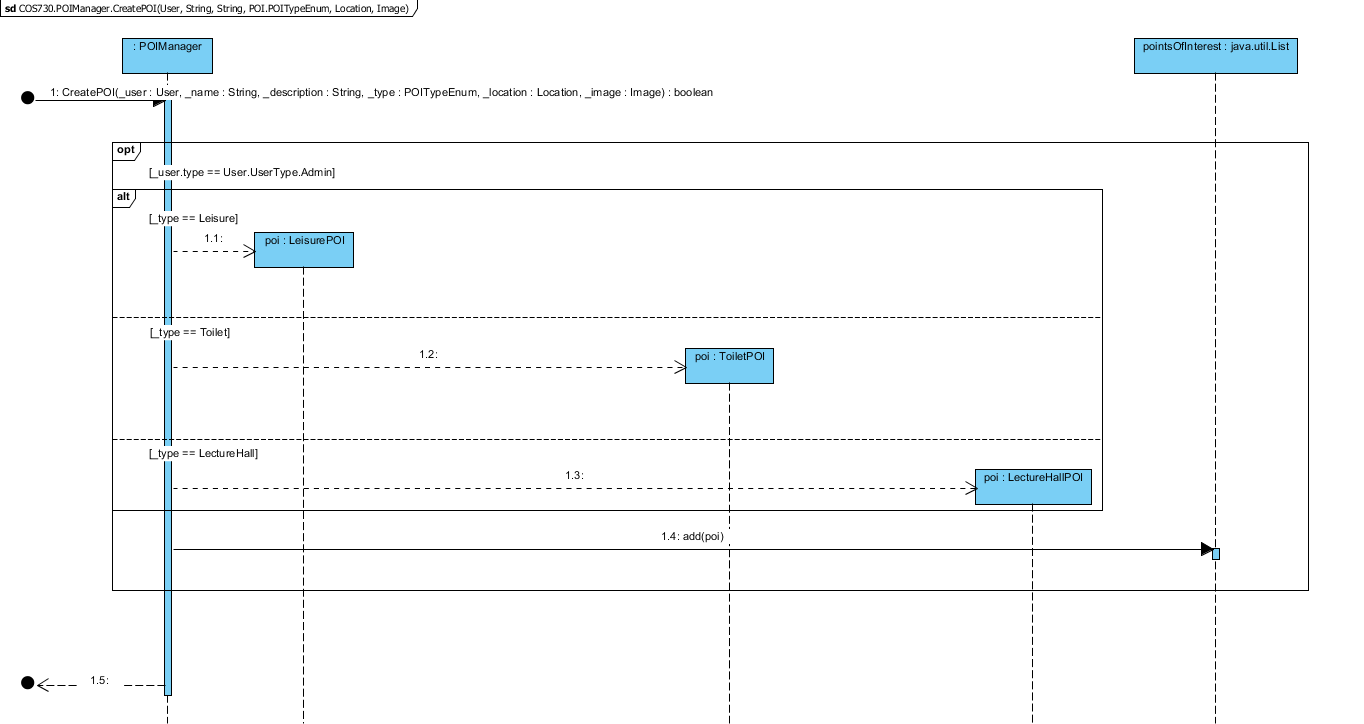
\includegraphics[width=\textwidth]{Images/CreatePOI_Sequence.png}
\caption{Sequence Diagram for the CreatePOI function}
\end{figure}

\begin{figure}[!htb]
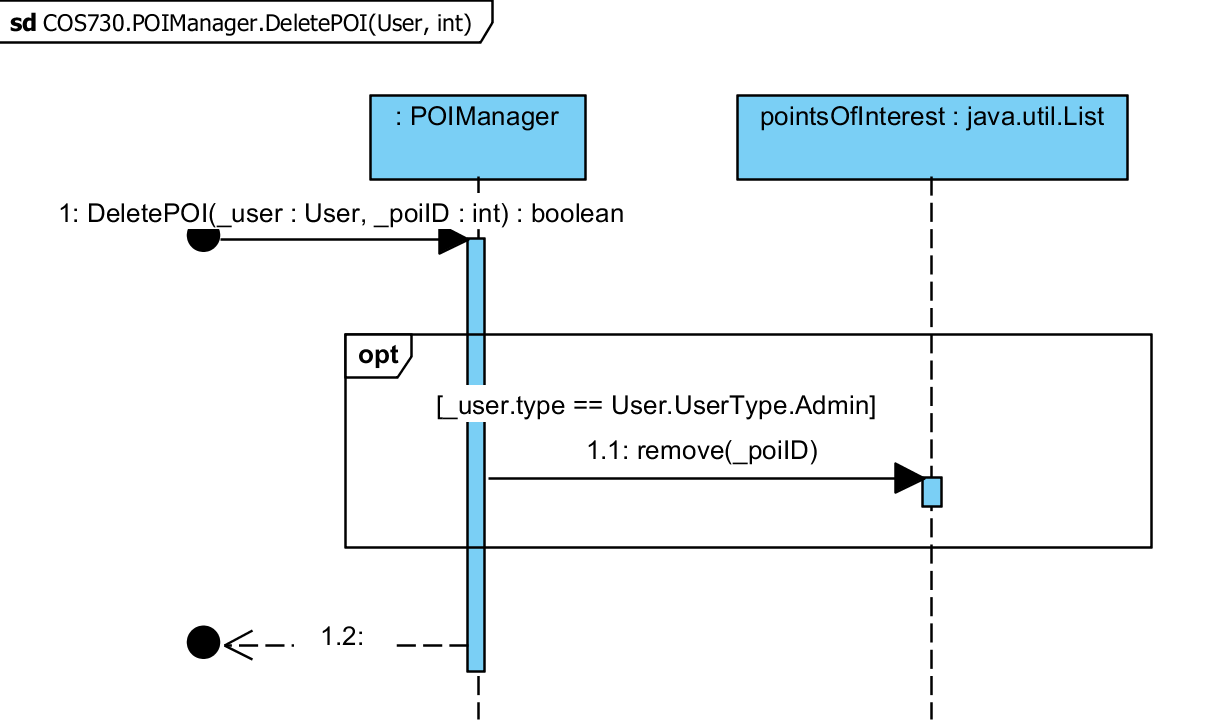
\includegraphics[width=\textwidth]{Images/DeletePOI_Sequence.png}
\caption{Sequence Diagram for the DeletePOI function}
\end{figure}

\begin{figure}[!htb]
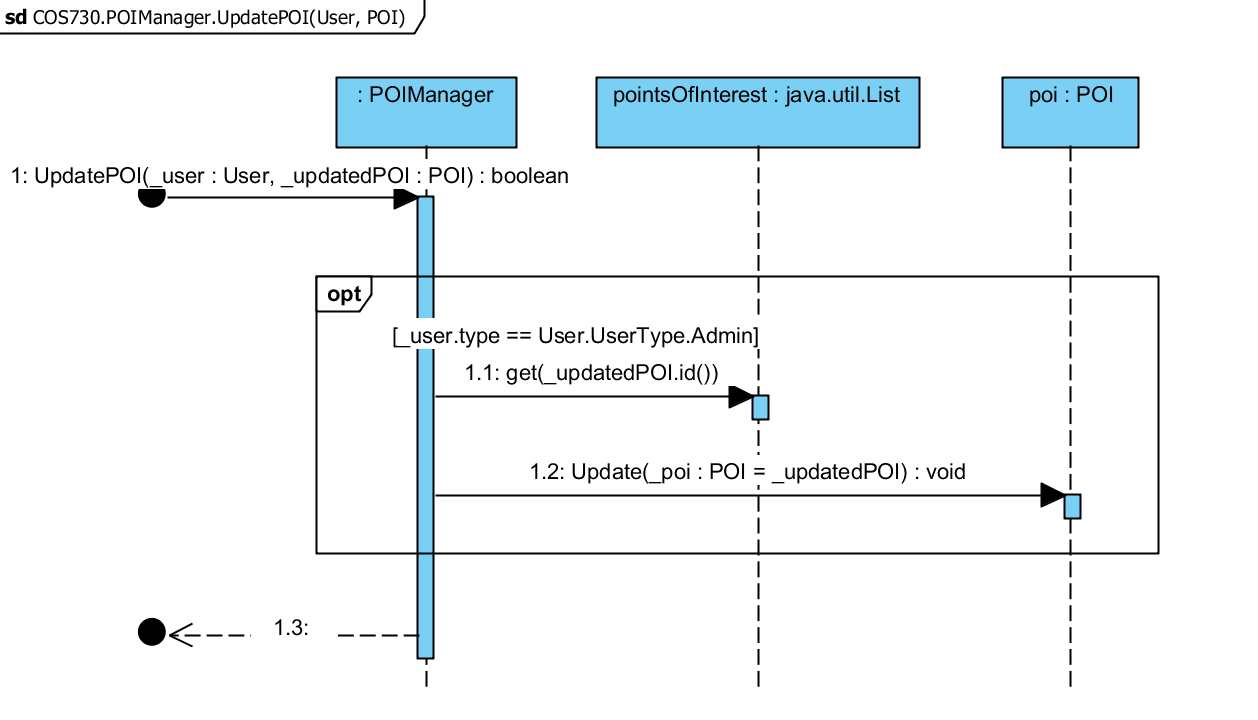
\includegraphics[width=\textwidth]{Images/UpdatePOI_Sequence.png}
\caption{Sequence Diagram for the UpdatePOI function}
\end{figure}

\begin{figure}[!htb]
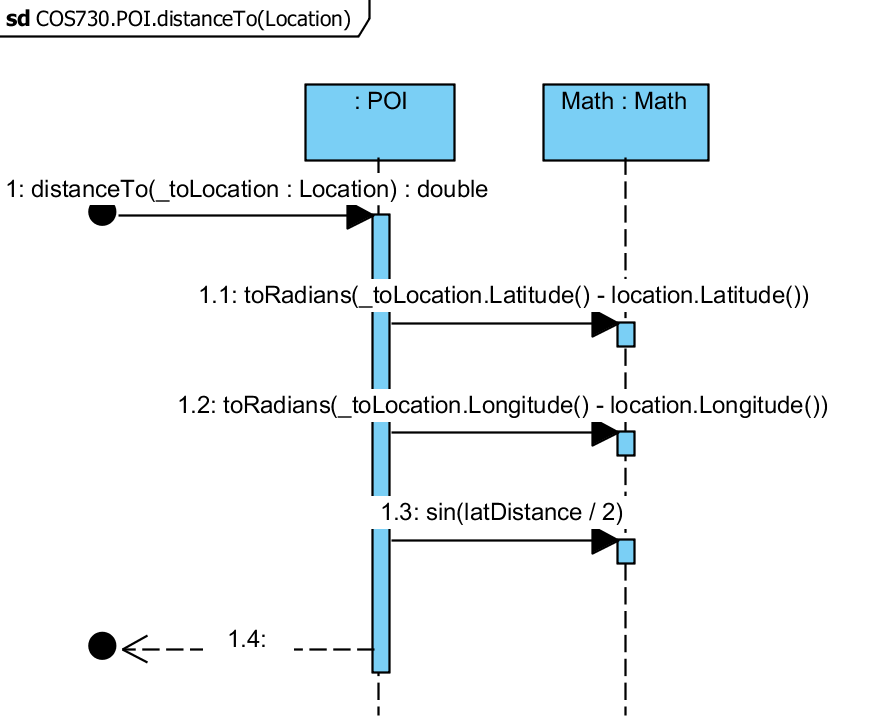
\includegraphics[width=\textwidth]{Images/DistanceTo_Sequence.png}
\caption{Sequence Diagram for the DistanceTo function}
\end{figure}

\begin{figure}[!htb]
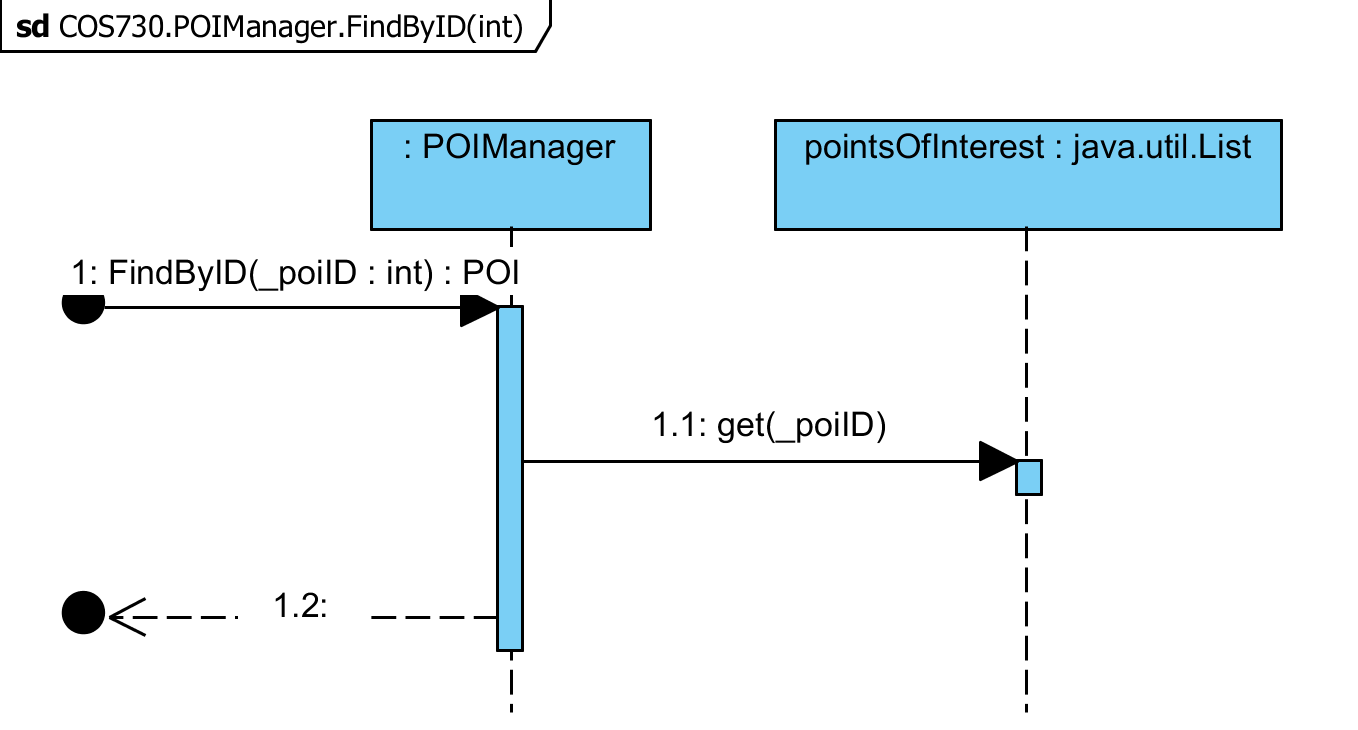
\includegraphics[width=\textwidth]{Images/FindByID_Sequence.png}
\caption{Sequence Diagram for the FindByID function}
\end{figure}

\begin{figure}[!htb]
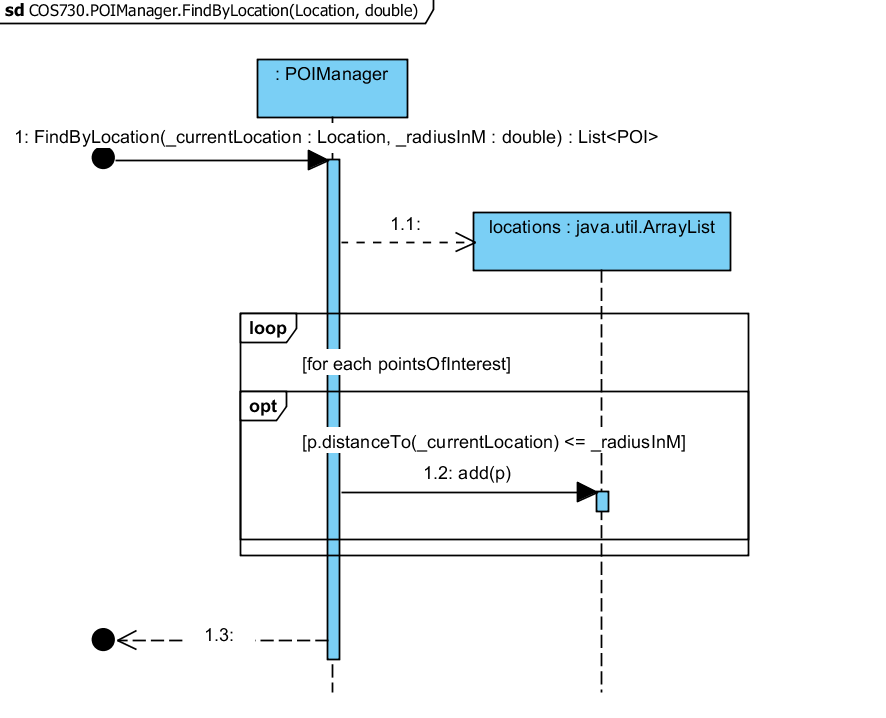
\includegraphics[width=\textwidth]{Images/FindByLocation_Sequence.png}
\caption{Sequence Diagram for the FindByLocation function}
\end{figure}

\begin{figure}[!htb]
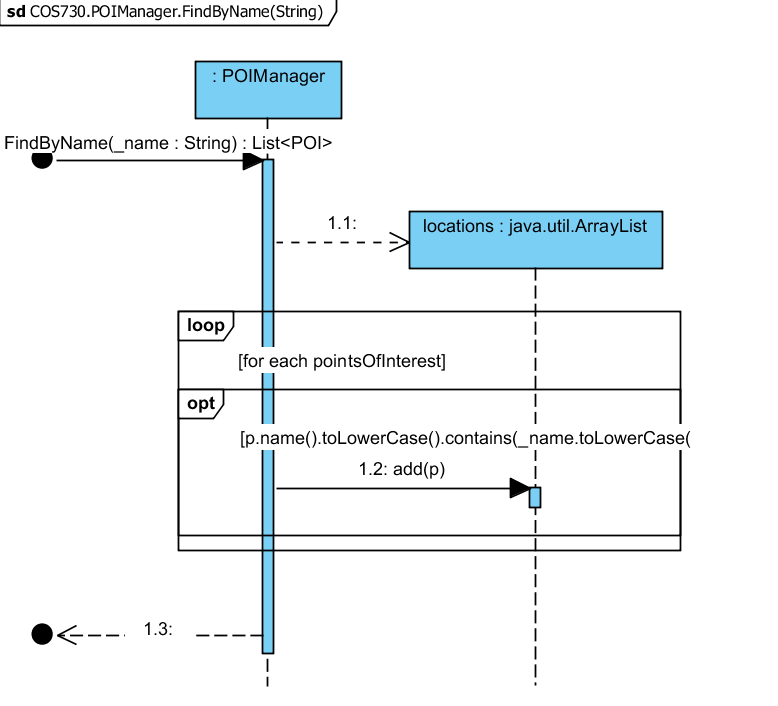
\includegraphics[width=\textwidth]{Images/FindByName_Sequence.png}
\caption{Sequence Diagram for the FindByName function}
\end{figure}

\begin{figure}[!htb]
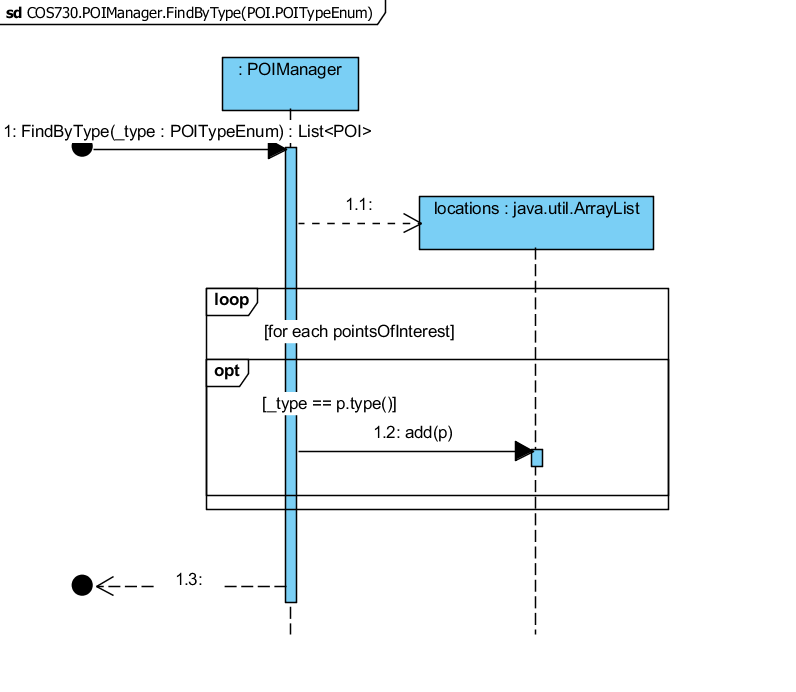
\includegraphics[width=\textwidth]{Images/FindByType_Sequence.png}
\caption{Sequence Diagram for the FindByType function}
\end{figure}

\begin{figure}[!htb]
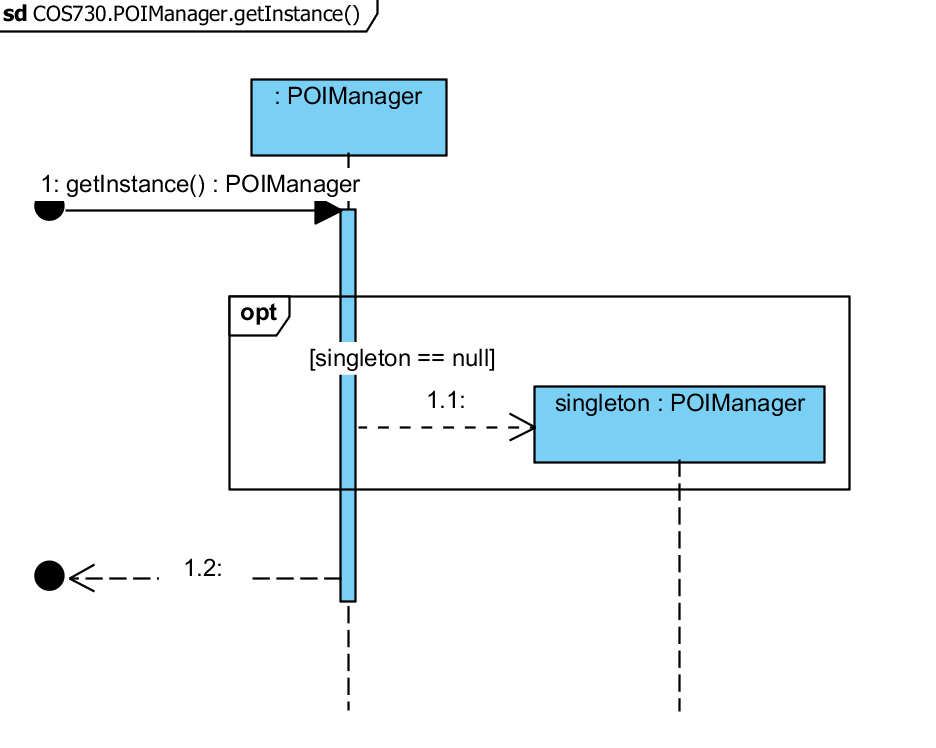
\includegraphics[width=\textwidth]{Images/getInstance_Sequence.png}
\caption{Sequence Diagram for the getInstance function}
\end{figure}

%%%%%%%

\section{Events Module}
\subsection{UML Class Diagram}
\includegraphics[width = \textwidth, height = 10cm]{ClassEvent}
\subsection {Use Case Diagram}

\subsection{Architectural Design of Module}
\paragraph{}The events module will be able to inform different users about events on campus. The module will make use of the location services of the navigation system, thus when a user passes a particular point of interest which has public events, the user will receive a notification via sms or email about these events. 

\paragraph{} The NavUP system will make use of a variety of design patterns. In the events module there will be an events superclass which abstracts the core fuctionality and members that an event object will provide. This means it will be possible to specify different events based on the type, i.e. a special lecture, exhibition, performance etc. In order to add functionality to these different types of events, the decorator design pattern will be used. A concrete decorator will be define to implemnt core funtionality defined by the abstarct event class, and the decorator class will hold a reference to an event object which to which functionality can be added dynamically.

\paragraph{} A single event object will have 4 different attributes namely a name for the event, a date, a time, and a location which is a Point of Intereste object. Different subcalsses will have addiotional attributes, such as a special lecture having a lecturers attribute, performances having performers information, and exhibitions having a topic description. The decorator pattern will allow us to add additional functionalities to each subclass based on the additional attributes which enhances specificity. 

\paragraph{} Each concrete event class will also be equiped with a Serialization function which will return the string containing information about the event which will be used in the notifaction that is sent to the user, which in the end is the goal of the module.  

\subsection{Technologies Used}
\paragraph{}


\subsection{Non-Trivial Implementation Tasks}
\paragraph{} The events module will be accessed when the user is using the NavUP system to navigate the UP campus. The system will continuously get the current location of the student and when a student passes a point of interest the system will check for events at the particular location. These events will then be compiled into a notification that the user will receive either as an SMS, email, or both. Once a notification has been sent the system will return to tracking the users location if the user is still using the system for navigation.\\
\newline
\includegraphics[width = \textwidth, height = 7cm]{EventsActivity}



\end{document}
